%!TEX root = ../bachelors_thesis.tex
\section{Model Overview}
Finding a good model design for this algorithm proved a rather hard task. I ended up with a few model classes in a traditional sense and the inevitable helper class that contains a bunch of static methods. I think for a clean design all of the source code would best be put in one, or at most two classes and be shipped as a single module. As can be seen in the simplified UML presented below the interaction between the classes is very limited and usually only one-way. They mainly serve the purpose to hide complicated code and provide a certain level of abstraction and modularity. For that reason all or most of it could be included in the master class \texttt{ProofSearch}. But I find it more comfortable to browse through different files of code than to have it all clustered up in one big file.

I believe that the reason for this situation of design is the fact that the code represents a single algorithm and thus is not as intuitive to break into smaller pieces. 

On the other hand it should be pointed out that it would be possible to structure this project in a more object-oriented style. But reimplementing it would probably cost more time and effort than would be won by doing so.

\subsection{Operation Syntax Tree}
One of the earliest challenges was to find a useful representation of formulas with which I could work decently. 

I looked through different Python libraries, but those I considered didn't fit my purpose. It was in this process of searching that I stumbled over the possibility to use binary trees to represent the syntax of a mathematical formula. Remembering what I learned in the lecture \emph{Datastructures and Algorithms} I realized that binary trees enable me not only to represent, but also to manipulate formulas as needed.

I decided to implement my own tree for that purpose. It might be argued that a lot of work could have been saved if I had used available syntax trees libraries, but I relished the idea of implementing a tree structure that I would use myself. Finally, I would put to use what I have learned in that lecture. I would have to make custom changes to a finished solution anyway and those changes probably would have been more work than the implementation of a binary tree. I tried to keep the tree as simple as possible, giving only a value to the nodes without supplying a unique key. The greatest challenge given by implementing a syntax tree was the handling of a unary operator. Braces serve to determine the depth of a tree, wherein a binary operator tells us when to start climbing up again. However, the unary introspection operator required additional case handling. 

The tree was not only important to the algorithm, but could also be used to check if the input was written correctly.

\subsection{Classes}

\subsubsection[Tree and Node]{\texttt{Tree} and \texttt{Node}}
As seen in the previous section I use a binary tree to represent, search, and manipulate formulas. The class \texttt{Tree} and the associated class \texttt{Node} are simple implementations of a syntax tree made to precisely fit my purpose. 

\begin{figure}[H]
	\caption{Simplified UML graphic of the classes used for implementing the algorithm. Additional helper methods and attributes are hidden.}
	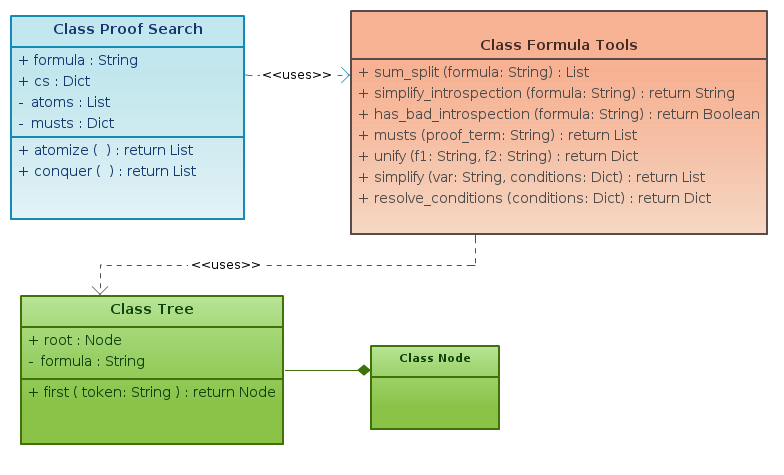
\includegraphics[width=1\textwidth]{Figures/uml_j-logic.png}
	\label{uml}
\end{figure}


\subsubsection[ProofSearch]{\texttt{ProofSearch}}
This class can be considered the core logic of this project. It takes the user input, evaluates the justification formula and finally returns whether the formula is provable or not. If it is, the output will also contain a proof.

\subsubsection[FormulaTools]{\texttt{FormulaTools}}
The name of the module already reveals its usage. This module doesn't wholly deserve to be called a class since it does not describe any model but simply serves as a box of tools which perform functions not solely related to the model \texttt{Tree} and \texttt{Node} nor to \texttt{ProofSearch}. It is something of an in-between. Removing this module would result in a lot of static methods where it would be unclear if they would best fit \texttt{Tree} or \texttt{ProofSearch}. Its core responsibility lies in modifying and analyzing formulas. This stands in contrast to the \texttt{Tree} class, which is only concerned with the single formula that it describes and the \texttt{ProofSearch} class, that does not actually handle formulas but only evaluates the result of an action on a formula and decides on how to proceed.


\section{Selected Methods}
In this section I want to show and explain some of the more important and thus more complicated methods that make up the heart of the algorithm. The source code of the methods presented here are excerpts only. Their in-line comments were shortened in order to keep the snippets as short as possible and to avoid unnecessary repetition. The aim of this section is to provide a insight into the source code without the need to read through all of it. 

\subsection[atomize]{\texttt{atomize, ProofSearch}}
The method \texttt{atomize} can be seen as the \emph{divide} step of the algorithm. I was tempted to name it such because it would have fit very nicely with the corresponding method \texttt{conquer} which will be presented here as well. I felt that the name \emph{atomize} carries more meaning than \emph{divide} and after all \emph{divide} and \emph{conquer} is more a general concept and does not fit this algorithm completely.

The method is a straightforward implementation of the algorithm in chapter~\ref{chap:Algorithm.divide}. It splits the formula for each sum operator found. Then it tries to simplify all subformulas that start with an introspection. Subformulas that are not resolvable~\footnote{Such as formulas that start with an introspection but cannot be simplified, or formulas that contain an introspection on the left side of an application.} are removed, leaving only those that we call \emph{atoms}.

\begin{figure}[H]
	\caption{Excerpt $atomize$ from $ProofSearch$.}
    \vspace{-10pt}
	\lstinputlisting[firstline=2, lastline=17]{Figures/code/atomize.py}
	\vspace{-10pt}
\end{figure}

\subsection[musts]{\texttt{musts, FormulaTools}}
The method \emph{musts} expects a given proof term to be atomized as it only distinguishes between introspection and application operators.
The algorithm takes the formula apart from top to bottom, generating new, smaller terms for every operator until the remaining proof term is but one proof constant. 

Since the resolution of an application operator introduces a new $X$ variable and the resolution of a introspection operator replaces an existing $X$ variable with a new one, the current $i$ for a new \emph{X-wild} $X_i$ is stored and increased in \texttt{v\_count}.

\begin{figure}[H]
	\caption{Excerpt $musts$ from $FormulaTools$}
    \vspace{-10pt}
	\lstinputlisting[firstline=2, lastline=20]{Figures/code/musts.py}
	\vspace{-10pt}
\end{figure}

If for example the current justification term is $((a\cdot (!b)):F)$, it will taken apart into the two subformulas $(a:(X_i\rightarrow F))$ and $((!b):(X_i))$. Further, since from $!b:X_i$ follows $\exists X_j \; s.t. \; !b:(b:X_j)$, all $X_i$ that occurred up until now must be replaced by $(b:X_j)$. These values are stored in \texttt{assignments} and eventually replaced.

In the end we will have only proof constants remaining.

\subsection[unify]{\texttt{unify, FormulaTools}}
I spent most of my time implementing this method, or rather its many predecessors. It used to be a lot longer and more complicated because it differentiated various cases concerning $X$ and $Y$ variables. In this final implementation, $X$ or $Y$ variables are handled the same on this level.

The method \texttt{unify} takes two formulas~\footnote{It is assumed that the only occurring operator are $\rightarrow$ and $:$. It would be easy to extend the code at this point.} and compares their tree structure. If the roots of both trees are operators and matching, the subtrees of both nodes are pushed on a stack to be further compared later. If one of the trees being compared is only a leaf and does not match the root of the other tree we either have found a contradiction or a \emph{condition}. In the first case the method will return \texttt{None}. In the other case, the term of the second tree becomes a \emph{condition} for the variable of the first tree.

All those conditions are stored as tuples in a set and are returned in form of a python dictionary, where all conditions for one variable can be accessed by the variable itself as a key. At the current stage conditions that apply to the same variable may contradict each other, but this method is responsible only for collecting conditions and not for evaluating them. This will done by the method \texttt{simplify} and the method \texttt{resolve\_conditions}.

\begin{figure}[H]
	\caption{Excerpt $unify$ from $FormulaTools$.}
	\vspace{-10pt}
	\lstinputlisting[firstline=2, lastline=25]{Figures/code/unify.py}
	\vspace{-10pt}
\end{figure}


\subsection[simplify]{\texttt{simplify, FormulaTools}}

The aim of this method is to replace all occurrences of the variable given as input except for its usage as key from the condition set.~\footnote{In the source code the condition on the variable is referred to as \emph{the chosen one}.}. 

For example, if we have $ (A \rightarrow B),\; (X_2),\; \text{and } (Y_1 \rightarrow Y_2)$ as conditions for $X_1$, and $(X_1)$ as a condition for $X_2$, the method returns $(A \rightarrow B)$ as the only condition for $X_1$, $(A \rightarrow B) \text{ and } (Y_1 \rightarrow Y_2)$ for $X_2$ and also $(A)$ for the new found variable $Y_1$ and $(B)$ for the new found variable $Y_2$. Thus we have eliminated all occurrences of the variable $X_1$ and as a consequence of this we found new variables that were not present before.

Implementing this method proved harder than expected because I underestimated the significance of the newfound variables. The method \texttt{resolve\_conditions} handles the order in which \texttt{simplify} is called on each variable. \texttt{resolve\_conditions} pushes the newfound variables on top of the stack to make sure they are given priority. Because \texttt{resolve\_conditions} needs to know the new variables, the method \texttt{simplify} makes changes to the condition set in place and instead of returning the conditions as might be expected, it returns the list of newfound variables.

\begin{figure}[H]
	\caption{Excerpt $simplify$ from $FormulaTools$.}
	\vspace{-10pt}
	\lstinputlisting[firstline=13, lastline=39]{Figures/code/simplify.py}
	\vspace{-10pt}
\end{figure}


\subsection[conquer]{\texttt{conquer, ProofSearch}}
Although the method \texttt{conquer} is the one returning the final result, the actual work is done by the method \texttt{conquer\_one\_atom}. As the name suggests it checks the provability of one atom only. \texttt{conquer} then simply summarizes the result of each atom and gives a readable output.

There are two main loops in \texttt{conquer\_one\_atom}. The first loop collects all possible configurations for each of the \emph{musts} of the atom. If for any \emph{must} no valid configuration can be found, the method will terminate because one unprovable \emph{must} makes the whole atom unprovable.

\begin{figure}[H]
	\caption{First excerpt $conquer\_one\_ atom$ from $FormulaTools$.}
	\vspace{-10pt}
	\lstinputlisting[firstline=3, lastline=19]{Figures/code/conquer.py}
	\vspace{-10pt}
\end{figure}

The second loop then tries to find an overall configuration that is compatible with at least one of the configurations per \emph{must}. If at one stage there is no entry left in \texttt{merged\_conditions}, it means that the conditions posed by the newly encountered configuration of the musts are not compatible with the old ones and thus the atom is unprovable.

\begin{figure}[H]
	\caption{Second excerpt $conquer\_one\_ atom$ from $FormulaTools$.}
	\vspace{-10pt}
	\lstinputlisting[firstline=23, lastline=41]{Figures/code/conquer.py}
	\vspace{-10pt}
\end{figure}

\bigskip


\section{Tests}
The simple unit tests I have written for this algorithm have been most important to its success. They served me in two ways: First to check if my code would behave and actually do what I expected. Second, when I encountered an example where I did not know what to expect, I would simple write a test for it and see what happened. This helped me understand the problem.
It is because of the tests that I have found so many mistakes, some minor, others major, making me re-code bits and parts again and again at a stage when I had hoped to be done with coding.

As can be seen when looking at the source code, not all all methods are tested on a same level of quality. Methods that I deemed simple usually have only one or two tests. An example for that is \texttt{summarize} from \texttt{ProofSearch}. This method simply rearranges the elements of a dictionary and returns a nice, readable output summarizing the content of the original input. In contrast to this, \texttt{\_\_str\_\_} from \texttt{Tree} which tests if the parsing of a formula works correctly contains lots of tests.

There are currently\footnote{Even though the program is finished I might add more tests to get rid of any doubts.} a total of 66 tests, almost half of which are related to \texttt{ProofSearch}. 